\documentclass[crop,tikz]{standalone}
\usepackage{tikz}
	\usetikzlibrary{shapes}
	\usetikzlibrary{automata}
	\usetikzlibrary{arrows}
	\usetikzlibrary{backgrounds}
	\usetikzlibrary{calc}
	\usetikzlibrary{positioning}
	\usetikzlibrary{patterns}
	\usetikzlibrary{decorations.pathmorphing}
	\usetikzlibrary{decorations.pathreplacing}

	
\input{../../../../../resources/latex/symbols.qmd}
\begin{document}

\begin{tikzpicture}

	\pgfdeclarelayer{background layer}
	\pgfdeclarelayer{foreground layer}
	\pgfsetlayers{background layer,main,foreground layer}

	\node (2d) at (0,0) {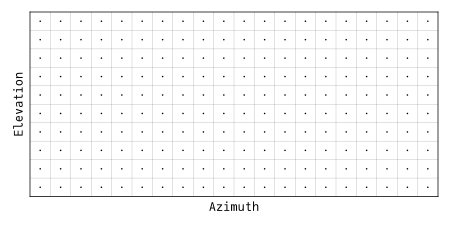
\includegraphics[natwidth=600px, natheight=300px]{./gs2dgrid_2d.pdf}};
	\node[below right = -2 and -14 of 2d] (proj) {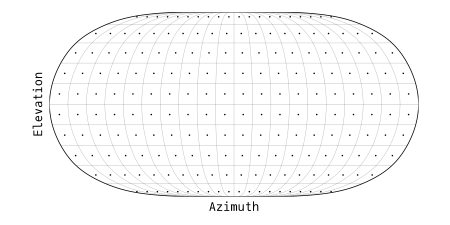
\includegraphics[natwidth=600px, natheight=300px]{./gs2dgrid_proj.pdf}};
	
	\begin{pgfonlayer}{background layer}
		\node[below right = -5.5 and -10 of proj] (3d) {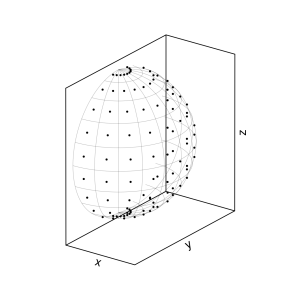
\includegraphics[natwidth=400px, natheight=400px, trim={0 30pt 0 0}, clip]{./gs2dgrid_3d.pdf}};
	\end{pgfonlayer}

	\draw[-latex, very thick] ($(3d.90)+(0,-3)$) to [in=0, out=90] node[near end, above, yshift=40px]{\LARGE{spherical projection}} ($(2d.0)+(-4,0)$) ;
	
	\draw[-latex, very thick] (2d.220) to [in=180, out=270] node[near end, below, yshift=-30px]{\LARGE{cartesian projection}} (3d.190) ;

\end{tikzpicture}

\end{document}